\section{Architectural Design --- Code Organisation and  Separation of Concerns}
\label{sec:architecture}

% Server vs lock step game design
% Shared parts of implementation between client and server 
% Layout of project
% IO and pure separation

When coming from an OO background, one of the first problems encountered when embarking on a large FP project is how to organise and architect the code. There is a certain paucity of literature pertaining to this issue; and while there are many projects on Hackage that provide good examples, the principles behind them are not always clear.\sidenote{cf. Section \ref{sec:fp_review} on page \pageref{cf:code_organisation}. }

There are two related issues here. First is simply what files should have what code in them; and second, how to separate concerns effectively. These can be seen as quite separate issues, but it is helpful to consider them simultaneously here, as should become apparent.

Common practice in OO languages is to have one class per file\sidenote{See \url{www.oracle.com/technetwork/java/codeconv-138413.html} (rev. 1999) and \url{www.possibility.com/Cpp/CppCodingStandard.html\#cflayout} for example. (Accessed April 2013).} but it is not immediately clear what principle in FP should determine the contents of a file. The approach taken in the Serenity project is instead to allow \emph{form} to follow \emph{function} (no pun intended); that is, to allow the desired separation of concerns to drive the module layout --- adjusting as becomes necessary --- rather than a specific type of code concept.

The main separation of concern that every Haskell project is going to contain to some degree or another is between pure and impure code, and so the first thing to be considered in designing an architecture for a project should be how the connection and communication between these areas is going to be managed.
At first sight it would appear that almost all of what happens in a game is IO of some sort or another, but this is not the case. Code can be pure precisely when its output can be defined in terms of its arguments \emph{only}.\sidenote{This is a simplification, but will suffice for the purpose of this text. See \bibentry{menger1953ideas}.} Motion of a particle in space experiencing a force due to gravity, for example, can be defined in terms of pure code. The process of writing log entries into a file will not be, (although the code that designated the actual content of the entries could be).

This is all very well, but does not make it immediately clear how to break down a project's code. The approach taken during the design of Serenity's module structure, and the approach recommended by this guide, is to let the structure of the main loop of each runnable component guide the nature and interface of each module.

%%todo: Should the sidenote have a cf. in it?
To demonstrate how this works, consider the architecture of the Serenity project. As discussed elsewhere,\sidenote{Section \ref{sec:specv2} page \pageref{sec:specv2}.} the game uses a server-client model, but with none or very limited simulation clientside. There are therefore two runnable components, which will share some logic. Each main loop will therefore have two main impure parts: the receiving of IO over the network from the server or client, and local IO (be it output to the screen, logging, or input from the user).

It is clear that some data structure must exist that models the state of the game. Because no simulation takes place on the client, all the updates to this structure will be due to messages from the server. User interactions also need to generate messages \emph{to} the server. So the client loop will consist of reading input from the network and updating the game state, rendering the screen, then reading input from the user and sending output to the network.

\begin{marginfigure}
	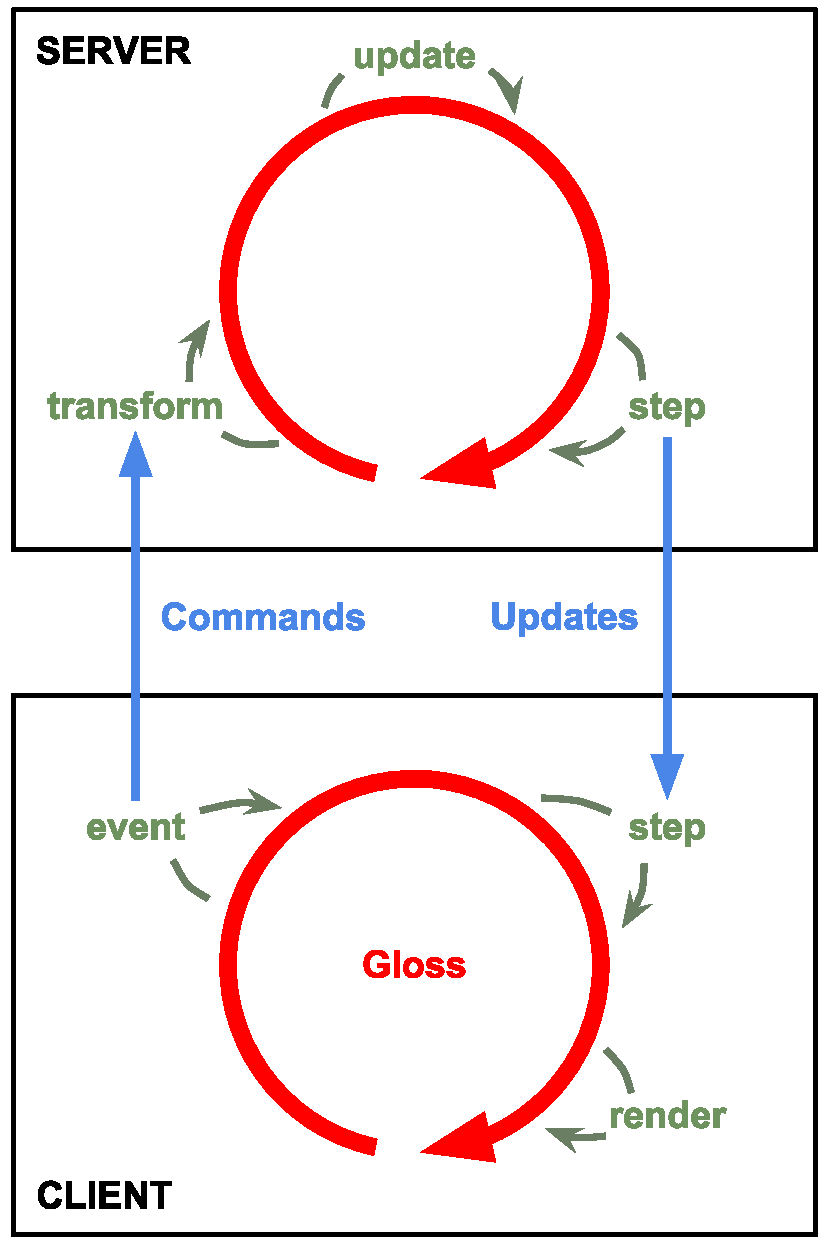
\includegraphics{res/architecture.pdf}
	\caption[Depiction of server and client main loops]{Depiction of server and client main loops. The main loops are in red, the network exchanges in blue, and pure function calls in green.}
	\label{fig:loops}
\end{marginfigure}

Conversely the server loop must read input from the clients and store it, simulate the game world and send the result of this simulation to all clients. Figure \ref{fig:loops} is a diagram of the interaction between these two loops.

From this simple analysis of the required basic functionality, several concepts have already been defined. On top of the loops themselves, there is:

\begin{itemize}\itemsep-3pt
    \item the network exchange (which comes in two flavours, client to server and server to client) 
    \item the game state itself
    \item the rules for updating the game state in reaction to updates from the server
    \item the rules for updating the game state in reaction to time passing (i.e.\ the simulation)
    \item The rules for rendering the screen
\end{itemize}

\begin{marginfigure}[6em]
	\begin{itemize}\parskip-3pt
    \item Game \begin{itemize}\itemsep-3pt
            \item Server
            \item Client
        \end{itemize}
    \item Model\begin{itemize}\itemsep-3pt
            \item Game state
            \item Time
        \end{itemize}
    \item Network
\end{itemize}
	\caption[The top level names in the module hierarchy in early versions of Serenity]{The top level names in the module hierarchy in early versions of Serenity.}
	\label{fig:loops}
\end{marginfigure}

\noindent It should be clear that this has immediately imparted a basic way of breaking up the project, and if we examine the top level module namespaces in the early versions of the Serenity source it can be seen that they correspond largely with the above list (the main difference being that the graphics code was contained within the Client modules). But it has also provided a guide to the IO/pure separation. The various parts of the game state, and the different ways in which it can be update (collectively referred to in the source as the \emph{model}) can be entirely pure. The network layer will clearly be impure, and can communicate representations of various aspects of the (pure) model.\sidenote{Bear in mind each of these headings does not need to --- and probably shouldn't --- represent one Haskell file. Instead they each represent  a top level module (rather like a package in Java) that is imported as one module but can be made up of several smaller internal modules.}

Surprisingly, the graphics logic is also entirely pure. This is because the code only has to define `what' to draw, in terms of an abstract "Picture" type. In the case of Serenity the actual impure drawing took place within the external library Gloss, but in projects where OpenGL (or similar) is used directly, it would still be wise to maintain this separation between a pure logic layer, and an impure `work' layer. This is an important and widely used concept, and is the subject of Section \ref{sec:pure}.

\paragraph{Summary of this section} Two important patterns have emerged during this discussion. Firstly there is the approach to setting out the top level breakdown of a large project: by considering units of functionality from the point of view of the main loop of the program and how these parts interface. This leads to both a decent module breakdown and a insight into the appropriate separation of pure and impure code.
